\documentclass[12pt]{article}
\usepackage[czech]{babel}
\usepackage[utf8]{inputenc}
\usepackage[plainpages=false,pdfpagelabels,unicode]{hyperref}
\usepackage[pdftex]{graphicx}
\usepackage[margin=2cm, includefoot]{geometry}
\usepackage{wrapfig}

\begin{document}

\title{Praktikum z patologické fyziologie \\
Vyšetření bariérové funkce kůže \\
Vyšetření kožní vodivosti}
\author{Marie Ostrá}
\maketitle

\section{Úvod}

Kůže zprostředkovává na převážné části povrchu lidského těla kontakt se zevním prostředím. Za
její bariérovou funkci je zodpovědná především nejsvrchnější vrstva epidermis, stratum corneum.
Bariérovou funkci kůže můžeme hodnotit tak, že kůži vystavíme určité definované zátěži a
sledujeme reakci kůže na zátěž, popřípadě měříme změny jejích fyzikálních a chemických
vlastností.

\begin{figure}[hb]
	\begin{centering}
	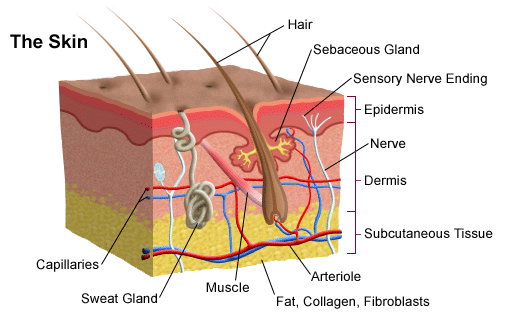
\includegraphics[width=0.7\linewidth]{kuze.png}
	\caption{Schéma kůže}
	\end{centering}
\end{figure}

\section{Postup}

Studenti provedou klasickou Burckhardtovu zkoušku.Ta spočívá ve sledování rozvoje erytému po
působení 0,5\,M roztoku NaOH jako standardní zátěži kožní bariéry. Poté provedou vyšetření
přístrojem Dermotest. Tady představuje standardní zátěž iontoforéza a stav kožní bariéry je
měřen jako kožní vodivost pří střídavém napětí o nízké frekvenci. Narušení kožní bariéry je
možné simulovat stržením povrchové vrstvy epidermis pomocí samolepící pásky nebo
odmaštěním kůže pomocí běžně používaných detergentů (SDS v prostředku na mytí nádobí).

\subsection{Burckhardtova zkouška}
Na volární stranu předloktí naneseme kapku 0,5\,M NaOH a překryjeme ji podložním sklíčkem.
Po 10\,min expozice posuzujeme makroskopicky stav pokožky pod okluzí. Pokud je zjevný
erytém, považujeme zkoušku za pozitivní (+++) příznak snížené funkce kožní bariéry. Pokud
erytém nevznikl, opakujeme expozici na dalších 10 min (vznik erytému po 20 min expozice-
pozitivita ++). Pokud erytém nevznikl, opakujeme expozici na dalších 10\,min (vznik erytému po
30 min expozice-pozitivita +). Pokud ani po 30\,min erytém nevznikl, považujeme zkoušku za
negativní. Tento výsledek svědčí o kvalitní bariérové funkci epidermis.

\subsection{Dermotest}
Přístroj Dermotest umožňuje měření elektrické vodivosti kůže při frekvenci střídavého proudu
32\,Hz v rozsahu 0--500\,$\mu$S. Metoda je kombinována s iontoforézou stejnosměrným proudem 1,5
mA, která představuje pro epidermis standardní zátěž. Přístroj ukládá do paměti 5 naměřených
hodnot vodivosti:
\begin{itemize}
	\item{V1 -- za 1 minutu po zahájení měření,}
	\item{V2 -- za 30\,s po zahájení iontororézy,}
	\item{V3 -- za 60\,s po zahájení iontoforézy,}
	\item{V4 -- za 30\,s po vypnutí iontoforézy,}
	\item{V5 -- za 60\,s po vypnutí iontoforézy.}
\end{itemize}
Indiferentní elektrodu obalíme gázou namočenou ve fyziologickém roztoku a položíme na ni
předloktí. Na volární stranu předloktí (vhodnou díky jemné vrstvě rohoviny v této oblasti a
64nízké hustotě potních žláz, které mohou výsledek měření modifikovat) přiložíme diferentní
elektrodu, podloženou kolečkem filtračního papíru, nasáklým fyziologickým roztokem. Po
stisknutí tlačítka START začíná 3 minuty trvající měření. Pět výše uvedených hodnot kožní
vodivosti V1-V5 je možno znovu vyvolat na displeji pomocí tlačítka VÝBĚR. Dermotestem
vyšetříme 10 posluchačů a 10 posluchaček.

\clearpage

\section{Výsledky}

\renewcommand{\arraystretch}{1.5}

\begin{table}[h]
	\begin{centering}
	\begin{tabular}{|c|c|}
	\hline
	Čas (s) & Stav pokožky \\
	\hline
	10 & \\
	\hline
	20 & \\
	\hline
	30 & \\
	\hline
	\end{tabular}
	\caption{Burckhardtova zkouška}
	\end{centering}
\end{table}

\begin{table}[h]
	\begin{centering}
	\begin{tabular}{|c|c|c|c|}
	\hline
	 & \multicolumn{3}{c|}{Vodivost ($\mu$S)} \\
	\hline
	Hodnota & bez narušení & narušení lepící páskou & narušení odmaštěním kůže \\
	\hline
	V1 & & & \\
	\hline
	V2 & & & \\
	\hline
	V3 & & & \\
	\hline
	V4 & & & \\
	\hline
	V5 & & & \\
	\hline
	\end{tabular}
	\caption{Dermotest}
	\end{centering}
\end{table}

\section{Závěr}

\end{document}
